% !TeX root = booklet-01.tex
\section{ساخت حافظه یک‌بیتی از گیت‌ها}
\label{sec:ch1-storage}
\subsection{چرا \lr{Feedback} لازم می‌شود؟}
خروجی مدار \lr{Combinational} پس از پایدارشدن، تابع ورودی جاری است؛
برای حفظ یک داده قدیمی باید اثری از حالت قبلی در مدار باقی بماند.
در ساختار ایستای این بخش، \lr{Feedback} خروجی را از مسیر گیت‌ها به ورودی برمی‌گرداند.
دو \lr{Inverter} پشت‌سرهم در حلقه، از نظر منطقی دو حالت سازگار دارند:
اگر یک گره صفر باشد، گره دیگر یک و بازگشت دوباره صفر است؛ حالت معکوس نیز ممکن است
\cite[بخش \secnum{۱.۴.۹}]{weste}.
این استدلال منطقی، زمان راه‌اندازی، نویز یا \lr{Metastability} را تحلیل نمی‌کند.
حالت اولیه بدون نوشتن داده یا مدار مقداردهی، لزوماً از پیش معلوم نیست.

\subsection{\lr{D Latch} با \lr{MUX} و دو \lr{Inverter}}
در شکل \ref{fig:ch1-latch}، یک \lr{MUX} بین ورودی تازه \(D\) و بازگشت
خروجی \(Q\) انتخاب می‌کند. پس از \lr{MUX} دو \lr{Inverter} داریم؛
آن‌ها سطح را بازسازی می‌کنند و مجموع اثر منطقی‌شان غیرمعکوس است.
برای \(E=1\)، ورودی تازه انتخاب و برای \(E=0\)، بازخورد انتخاب می‌شود
\cite[شکل \secnum{۱.۳۱}]{weste}.

\begin{figure}[ht]
\centering
\begin{latin}
\begin{tikzpicture}[x=1cm,y=1cm]
\draw (0,0)--(0,2)--(1.2,1.7)--(1.2,0.3)--cycle;
\node at (0.55,1.35) {$D$};\node at (0.55,0.65) {$Q$};
\draw[->] (-1.4,1.4) node[left] {$D$}--(0,1.4);
\draw (1.2,1)--(2,1);
\draw (2,0.6)--(2,1.4)--(2.7,1)--cycle;\draw (2.78,1) circle (0.08);
\draw (2.86,1)--(3.5,1);
\draw (3.5,0.6)--(3.5,1.4)--(4.2,1)--cycle;\draw (4.28,1) circle (0.08);
\draw[->] (4.36,1)--(5.9,1) node[right] {$Q$};
\draw (5.1,1)--(5.1,-1)--(-0.8,-1)--(-0.8,0.6)--(0,0.6);
\fill (5.1,1) circle (1.5pt);
\draw[->] (0.6,3) node[above] {$E$}--(0.6,1.85);
\node at (0.5,2.3) {MUX};
\node[above] at (2.9,1.2) {$\overline{Q}$};
\end{tikzpicture}
\end{latin}
\caption{بازترسیم بلوکی \lr{Latch} مثبت‌حساس بر پایه کتاب \cite{weste}.
در \lr{MUX}، \(E=1\) ورودی \(D\) و \(E=0\) بازخورد \(Q\) را انتخاب می‌کند.
نام گره میانی \(\overline{Q}\) معنای منطقی پایدار آن را نشان می‌دهد.}
\label{fig:ch1-latch}
\end{figure}

رابطه حالت در مدل منطقی چنین است:
\begin{equation}\label{eq:ch1-latch}
Q_{\mathrm{next}}=ED+\overline{E}Q_{\mathrm{current}}.
\end{equation}
برای \(E=1\)، رابطه به \(Q_{\mathrm{next}}=D\) تبدیل می‌شود؛
تا وقتی فعال‌ساز یک است، خروجی پس از تاخیرهای مدار تغییر ورودی را دنبال می‌کند.
این حالت \lr{Transparent} است؛ \lr{Latch} فقط در لحظه بالا رفتن \(E\) نمونه نمی‌گیرد.
برای \(E=0\)، داده تازه جدا و حلقه بازخورد بسته می‌شود؛
رابطه به \(Q_{\mathrm{next}}=Q_{\mathrm{current}}\) تبدیل می‌شود و داده حفظ می‌شود.
به این حالت \lr{Opaque} می‌گوییم.

در پیاده‌سازی \lr{TG}، مسیر ورودی با \(E\) و مسیر بازخورد با \(\overline{E}\)
فعال می‌شود؛ دو کنترل مکمل باید هر دو مسیر را هماهنگ کنند.
با دو \lr{TG} و دو \lr{Inverter}، هسته هشت ترانزیستور دارد؛
این شمارش تولید مکمل کنترل و مدارهای جانبی را شامل نمی‌شود.
وجود دو \lr{Inverter} باعث می‌شود نگهداری صرفاً به بار یک خازن جداافتاده متکی نباشد؛
در مدل ایستای تغذیه‌شده، بازخورد حالت را بازتولید می‌کند.

\subsection{جدول زمانی آموزشی برای \lr{Latch}}
جدول \ref{tab:ch1-latch-time} یک توالی مستقل آموزشی است.
حالت اولیه صفر فرض شده و میان رویدادها زمان کافی برای پایدار شدن داریم.
\begin{table}[ht]
\centering
\caption{ردگیری یک \lr{Latch} مثبت‌حساس؛ هر ردیف وضعیت پس از رویداد را نشان می‌دهد.}
\label{tab:ch1-latch-time}
\begin{tabular}{cccp{7cm}}
\toprule
\(E\)&\(D\)&\(Q\)&توضیح\\
\midrule
۰&۰&۰&حالت اولیه فرض‌شده نگه داشته می‌شود.\\
۱&۰&۰&مسیر داده باز می‌شود؛ خروجی صفر است.\\
۱&۱&۱&بدون لبه تازه فعال‌ساز، تغییر داده عبور می‌کند.\\
۰&۱&۱&مسیر داده بسته و یک نگه داشته می‌شود.\\
۰&۰&۱&داده تغییر کرده است؛ خروجی نگه داشته می‌شود.\\
\bottomrule
\end{tabular}
\end{table}
این جدول تفاوت حساسیت به سطح و حساسیت به لبه را نشان می‌دهد.
با عوض کردن ورودی‌های \lr{MUX}، می‌توان \lr{Latch} منفی‌حساس ساخت:
آن‌گاه وقتی کنترل صفر است شفاف و وقتی یک است نگهدارنده خواهد بود.

\subsection{\lr{D Flip-Flop} از دو \lr{Latch} مکمل}
یک \lr{Latch} منفی‌حساس را \lr{Master} و پس از آن یک \lr{Latch}
مثبت‌حساس را \lr{Slave} قرار می‌دهیم.
هر دو از همان \lr{Clock} به نام \(CLK\) استفاده می‌کنند، ولی فعال‌ساز
اولی \(\overline{CLK}\) و دومی \(CLK\) است
\cite[شکل \secnum{۱.۳۲}]{weste}.
شکل \ref{fig:ch1-flop} مسیر داده را نشان می‌دهد.

\begin{figure}[ht]
\centering
\begin{latin}
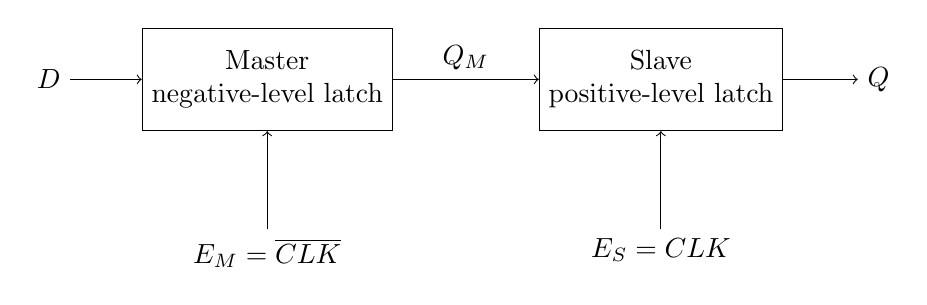
\begin{tikzpicture}[x=1cm,y=1cm]
\node[draw,minimum width=2.8cm,minimum height=1.3cm,align=center] (m) at (0,0)
{Master\\negative-level latch};
\node[draw,minimum width=2.8cm,minimum height=1.3cm,align=center] (s) at (5,0)
{Slave\\positive-level latch};
\draw[->] (-2.5,0) node[left] {$D$}--(m.west);
\draw[->] (m.east)--node[above] {$Q_M$} (s.west);
\draw[->] (s.east)--(7.5,0) node[right] {$Q$};
\draw[->] (0,-1.9) node[below] {$E_M=\overline{CLK}$}--(m.south);
\draw[->] (5,-1.9) node[below] {$E_S=CLK$}--(s.south);
\end{tikzpicture}
\end{latin}
\caption{ساختار آموزشی \lr{Master--Slave Flip-Flop} لبه‌بالارونده.
هر بلوک یک \lr{Latch} است؛ پیکان‌های پایین فقط کنترل شفاف بودن‌اند.}
\label{fig:ch1-flop}
\end{figure}

سه وضعیت را جدا بررسی می‌کنیم:
\begin{enumerate}
\item \textbf{هنگام صفر بودن \lr{Clock}:}
\lr{Master} شفاف است و \(Q_M\) داده \(D\) را دنبال می‌کند؛
\lr{Slave} بسته است و خروجی قبلی \(Q\) را نگه می‌دارد.
پس تغییر \(D\) در این فاز فوراً به \(Q\) نمی‌رسد.
\item \textbf{در گذار صفر به یک:}
\lr{Master} بسته و مقدار داده نزدیک این لبه را نگه می‌دارد؛
\lr{Slave} باز می‌شود و آن مقدار ذخیره‌شده را به \(Q\) می‌رساند.
پس از تاخیر انتشار، خروجی با نمونه ثبت‌شده برابر می‌شود.
\item \textbf{هنگام یک بودن و سپس افت \lr{Clock}:}
در فاز یک، تغییر بعدی \(D\) از \lr{Master} بسته عبور نمی‌کند.
در لبه افت، \lr{Slave} بسته و خروجی را نگه می‌دارد؛
\lr{Master} دوباره برای نمونه بعدی باز می‌شود.
\end{enumerate}
در مدل ایدئال، این رفتار با ثبت \(D\) در لبه بالارونده معادل است؛
دو \lr{Latch} هم‌حساس چنین جداسازی فازهایی ندارند و ممکن است مسیر شفاف سرتاسری بسازند.
با جابه‌جا کردن قطبیت دو \lr{Latch}، \lr{Flip-Flop} لبه‌پایین‌رونده ساخته می‌شود.

\subsection{نمونه‌برداری لبه‌ای، حالت اولیه و محدودیت زمانی}
فرض کنید \(Q\) ابتدا صفر است و \(D\) پیش از لبه اول یک شده و پیرامون لبه
پایدار می‌ماند. در لبه اول، خروجی پس از تاخیر انتشار یک می‌شود.
اگر \(D\) میان دو لبه به صفر برسد، خروجی تا لبه بعدی یک می‌ماند؛
به شرط رعایت محدودیت‌های زمانی، در لبه بعدی صفر ثبت می‌شود.
بدون تعیین داده ثبت‌شده یا مقداردهی اولیه، \(Q\) را نباید خودبه‌خود صفر فرض کرد.

در مدار واقعی، داده باید پیش از لبه برای مدت \lr{Setup Time} و پس از آن برای
مدت \lr{Hold Time} پایدار بماند. این اصطلاح‌ها به پنجره اطمینان ثبت مربوط‌اند؛
نقضشان ممکن است خروجی نامطمئن ایجاد کند.
\lr{Clock Skew} اختلاف زمان رسیدن ساعت به عناصر مختلف است و می‌تواند
شرایط نگهداری را تحت تاثیر قرار دهد \cite[ابتدای صفحه چاپی ۱۹]{weste}.
این بخش مقدار عددی هیچ‌یک را تعیین یا بی‌خطا بودن زمان‌بندی یک مدار واقعی را اثبات نمی‌کند.

\subsection{دو فاز غیرهم‌پوشان و \lr{Register}}
کتاب برای کاهش خطر شفاف بودن هم‌زمان مسیرهای دو مرحله، ساختاری با دو فاز
\(\phi_1\) و \(\phi_2\) غیرهم‌پوشان معرفی می‌کند
\cite[شکل \secnum{۱.۳۳}]{weste}.
منظور از غیرهم‌پوشان این است که دو فعال‌ساز هم‌زمان یک نباشند؛
میان آن‌ها می‌تواند فاصله‌ای باشد که هر دو صفرند.
در مدل \lr{Latch}، بنابراین دست‌کم یک مرحله بسته می‌ماند و مسیر شفاف کامل نداریم.
این نتیجه به حفظ قید غیرهم‌پوشانی در محل دریافت کنترل‌ها وابسته است؛
جای تحلیل همه محدودیت‌های واقعی و \lr{Setup Time} را نمی‌گیرد.

چند \lr{D Flip-Flop} با \lr{Clock} مشترک، یک \lr{Register} چندبیتی می‌سازند.
برای مثال، هشت \lr{Flip-Flop}، برداری هشت‌بیتی را در لبه ساعت ثبت می‌کنند.
وجود یک \lr{Clock} منطقی مشترک به معنی صفر بودن اختلاف تاخیر مسیرهای ساعت نیست.
بافرگذاری ورودی و خروجی برای ایجاد رابط مناسب میان ماژول‌ها نیز در پایان
بحث کتاب مطرح شده است؛ جزئیات \lr{Modularity} در ادامه فصل می‌آید.

\section{تمرین‌های تحلیلی و کنترل پوشش}
\subsection{پرسش‌ها}
\begin{enumerate}
\item چرا دو برابر شدن تعداد ترانزیستورها به معنی نصف شدن تاخیر هر مدار نیست؟
\item برای \(Y=\overline{A(B+C)}\)، شبکه بالا و پایین را تعیین و تعداد قطعات را بشمارید.
\item در \lr{AOI22} با \((A,B,C,D)=(0,1,1,1)\)، کدام مسیر خروجی را تعیین می‌کند؟
\item در یک \lr{MUX} دوورودی با \(D_0=1,D_1=0\)، تابع خروجی نسبت به \(S\) چیست؟
\item در \lr{Latch} مثبت‌حساس، اگر داده هنگام صفر بودن کنترل تغییر کند، خروجی چه می‌شود؟
\item آیا با سری کردن دو \lr{Latch} مثبت‌حساس با کنترل مشترک،
همان \lr{Flip-Flop} لبه‌ای قبلی را به دست می‌آوریم؟
\end{enumerate}

\subsection{پاسخ‌های تشریحی}
\begin{enumerate}
\item شمار ترانزیستور، مشخصه ساختار است؛ تاخیر به مسیر، جریان، ظرفیت، سیم‌ها و بار وابسته است.
مدل رشد تعداد به‌تنهایی هیچ‌یک از این وابستگی‌ها را حل نمی‌کند.
\item پایین، \lr{nMOS} کنترل‌شده با \(A\) را با گروه موازی \(B,C\) سری می‌کنیم.
بالا، \lr{pMOS} کنترل‌شده با \(A\) را با گروه سری \(B,C\) موازی می‌کنیم؛
شرط بالا \(\overline{A}+\overline{B}\,\overline{C}\) است.
سه ترانزیستور در هر شبکه و مجموعاً شش ترانزیستور داریم.
\item شاخه \(CD\) پایین کامل است؛ خروجی صفر می‌شود.
در بالا گروه \(C,D\) کاملاً قطع است، پس مسیر متضاد نداریم؛ روشن بودن بخشی از شبکه بالا کافی نیست.
\item از رابطه \eqref{eq:ch1-mux}، \(Y=\overline{S}\) به دست می‌آید.
برای \(S=0\)، ورودی اول یک و برای \(S=1\)، ورودی دوم صفر انتخاب می‌شود.
\item مسیر ورودی تازه قطع است و حلقه بازخورد مقدار قبلی را نگه می‌دارد؛
اگر حالت اولیه معلوم نباشد، از این رویداد به‌تنهایی مقدار خروجی معلوم نمی‌شود.
\item خیر؛ در فاز یک، هر دو شفاف‌اند و داده می‌تواند از هر دو عبور کند.
ساختار معرفی‌شده به قطبیت مکمل دو مرحله و زمان‌بندی مناسب نیاز دارد.
\end{enumerate}

\subsection{آنچه اکنون باید بتوانید توضیح دهید}
بخش \secnum{۱.۱} رشد مجتمع‌سازی و محدودیت تفسیر آمار تاریخی را معرفی کرد؛
بخش \secnum{۱.۲} مسیر تابع تا مدار و شکل فیزیکی را نشان داد؛
بخش \secnum{۱.۳} ساختار و مدل مقدماتی \lr{MOS} را توضیح داد.
در بخش \secnum{۱.۴} همه زیربخش‌ها از \lr{Inverter} تا گیت‌های
\lr{Compound}، مسیرهای عبوری، \lr{Tristate}، \lr{MUX} و عناصر حافظه بررسی شدند.

برای تحلیل یک مدار تازه، نوع قطعات، کنترل‌ها، مسیر داده و شرایط مدل را جدا بنویسید.
سپس برای ورودی‌های موردنظر مسیر کامل تا هر ریل را دنبال و وجود خروجی شناور یا
هدایت متضاد را کنترل کنید. در عنصر حافظه‌دار، حالت قبلی و فاز کنترل نیز لازم‌اند.
این روش از جدول درستی فراتر می‌رود و زمینه ورود به \lr{Fabrication}، \lr{Layout}
و مدل کمی ترانزیستور را فراهم می‌کند.
